\chapter{Einleitung}\label{einleitung}
\addthumb{Einleitung}{\huge{\textbf{\thechapter.}}}{white}{haw_rot} 

Im Jahr 1926 veröffentlitche der Wirtschaftswissenschaftler Nikolai D. Kondratieff (* 1892, \dag 1938) die Theorie \glqq Die Langen Wellen der Konjunktur\grqq \cite{hensen:gesundeGesellschaft}.
Leo Nefiodow erweiterte 2006 die Theorie, damit die Entwicklung des 20. Jahrhunderts einfließen konnte.\\
Kondratieff zeigte, dass sich die gesellschaftliche Wandlung nicht willkürlich vollzog. Seit der Industrialisierung Mitte des 18. Jahrhunderts stand der Wohlstand der Gesellschaft in direkter Beziehung zu besonderen Erfindungen. Er betrachtete die Phasen des Wohlstandes und die direkt folgende Wirtschaftskrise und entdeckte die später nach ihm benannten \glqq Kondratieff-Zyklen\grqq.
Wie in Abbildung \ref{zyklen} zu sehen ist, war die Dampfmaschine die erste Basisinnovation\footnote{Basisinnovationen müssen nach Nefiodow vier Eigenschaften erfüllen: Entstehung eines neuen Marktes mit vielen Arbeitsplätzen; Innovation bestimmt den Zyklus; Basisinnovationen haben einen Zyklus von 40 - 60 Jahren; Sie bestimmen die Entwicklungsrichtung} und revolutionierte die Textilindustrie.\cite{wieden:liquidwork}

%\begin{wrapfigure}{c}{10cm}
%\centering
%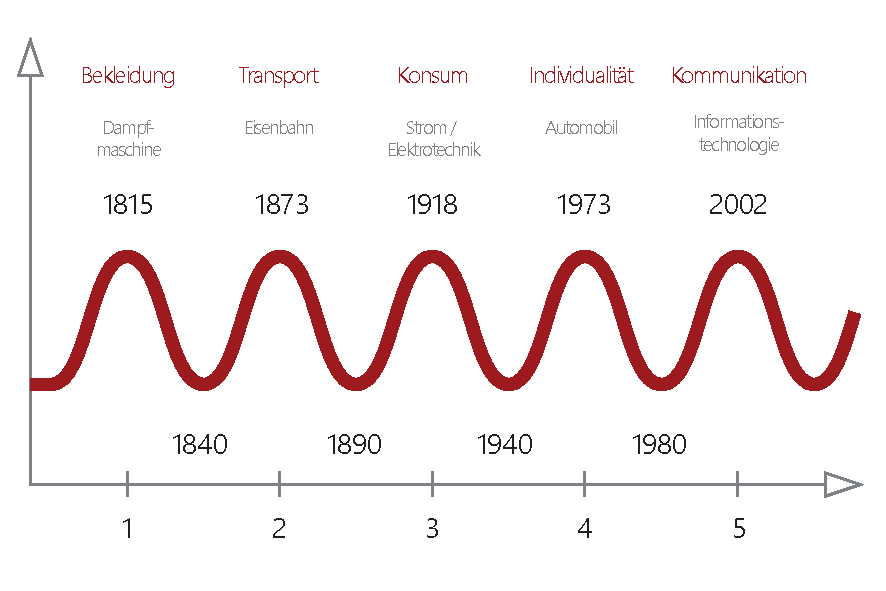
\includegraphics[width=8cm]{./img/zyklen.pdf}
%\caption{Kontratieff Zyklen}
%\label{zyklen}
%\end{wrapfigure}

\begin{figure}[htbp]
  \vspace{0.5cm}
  \centering
  \fbox{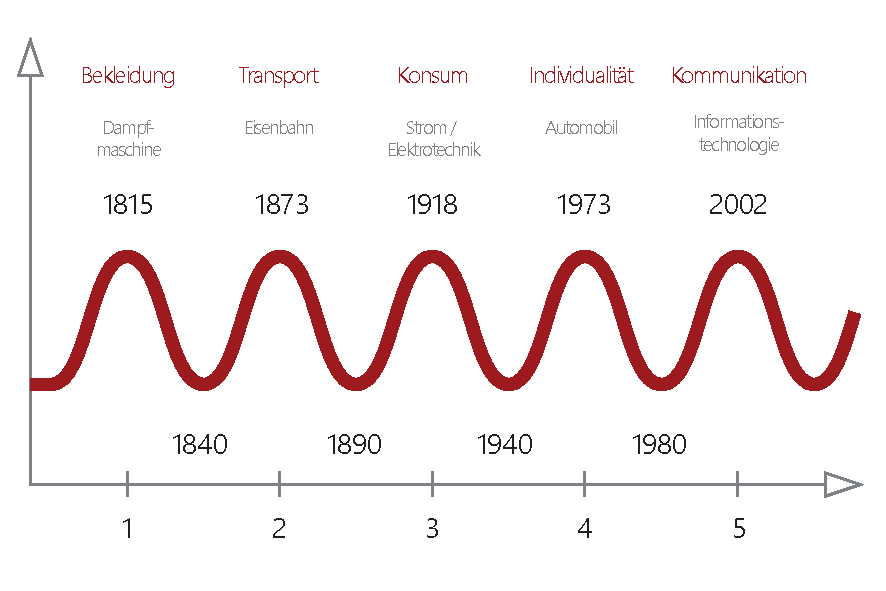
\includegraphics[angle=0,width=12cm]{./img/zyklen.pdf}}
  \caption{Kondratieff-Zyklen}
  \label{zyklen}
  \vspace{0.5cm}
\end{figure}

Diese Erfindung gilt als Beginn des ersten Kondratieff-Zyklus. Vor dem maschinellen Betrieb wurden Spinnräder noch manuell bedient und Kleidung war teuer. Die dampfbetriebenen Webstühle steigerten
die effizient um das 200-fache. In 20er Jahren stagnierte die Branche, da die Rohstoffbeschaffung und Warenverteilung das Maximum der Effizienz erreicht hatte. Mit der Erfindung der Eisenbahn gelang der Übergang vom ersten in den zweiten Zyklus. In den folgenden Jahren konnte nun das Bedürfnis nach verbesserten Transportmöglichkeiten gestillt werden.\\
Dampfmaschine, Eisenbahn, Strom, Motor und der Mikrochip stehen alle für eine Basisinnovation, die zukünftige Gesellschaften geprägt haben. Im lauf der Zeit verschwinden die Erfindungen aus dem Bewusstsein der Menschen und werden zu Gegenständen des Alltags. Motor und Mikrochip sind so stark im gesellschaftlichen Leben verankert, dass Sie nicht mehr direkt wahrgenommen werden. Betrachtet man eine elektrische Zahnbürste, ist es selbstverständlich, dass die Energie aus dem Stromnetz bezogen wird und der Bürstenkopf von einem Motor angetrieben wird.\\
Das Jahr 2002 gilt als Höhepunkt des fünften Kondratieff-Zyklus und die Gesellschaft befindet sich gerade im Übergang zum Sechsten. Noch fehlt die aktuelle Basisinnovation und auch das zu stillende Bedürfnis ist nach der Kommunikation noch nicht bestimmt.\\
Nach Nefiodow \cite{nefiodow:gesundheit} gibt es vier Möglichkeiten welcher Markt in Zukunft den sechsten Kondratieff prägen wird:
\begin{itemize}
  \item \textbf{Informationsmarkt} \\
  		Mobile Geräte und Soziale Netzwerke sind maßgebend für diesen Markt. So verhalf der Kurznachrichtendienst Twitter zum sogenannten \glqq Arabischen Frühling\grqq, durch die blitzschnelle Kommunikation über das Netz\footnote{http://www.heise.de/tr/blog/artikel/Wie-funktioniert-die-Twitter-Revolution-1761481.html \\aufgerufen am 06.01.2014}.
  \item \textbf{Bio - und Nanotechnologie} \\
  		Die Erfindung des Mikroskops und die Entschlüsselung der DNA im Jahr 2000 gilt als Basisinnovation. Anfangs wurden die Erkenntnisse nur in Medizin und Pharmazie angewendet. Heute profitiert auch die Landwirtschaft und Lebensmittelindustrie davon.
  \item \textbf{Umwelttechnologie}
  		Auch der Bereich Umwelttechnologie sorgte für einen Zuwachs an Arbeitsplätzen. In Deutschland standen im Bereich der erneuerbaren Energien 170.000 Menschen in einem Beschäftigungsverhältnis\footnote{vgl. \cite{nefiodow:gesundheit} S. 107}.
  \item \textbf{Gesundheit}
  		Der Gesundheitsmarkt vereint technologische Komponenten wie die Medizintechnik und psychosoziale Gesundheit. Es erfolgt ein Wechsel vom heutigen \glqq Krankheitswesen\grqq zum Gesundheitswesen, angefangen von der Burnout-Prophylaxe, Gesundheitstourismus zur Bionik und künstlichen computergesteuerten Prothesen.
\end{itemize}

\section{Gesundheit als sechster Kondratieff-Zyklus}

Nach Granig\cite{nefiodow:gesundheit} ist der Gesundheitsbereich der derzeit am schnellsten wachsende Markt\footnote{Gemessen am Anteil der Branche am Bruttoinlandsprodukt}. Die Bevölkerung ist gewillt in die eigene Gesundheit zu investieren und die Unternehmen positionieren sich im Gesundheitsbereich (Siemens beispielweise verstärkt sich im Bereich der Medizintechnik).
Die Bio- und Nanotechnologie ist und die Medizintechnik ähneln sich in einigen Bereichen. Sowohl Siemon Cord \cite{cord:innovation} als auch Granig\footnote{vgl. \cite{nefiodow:gesundheit} Seite 116 f} sprechen davon, dass der Markt sich nur gehemmt entwickeln kann. Grund dafür sind sowohl in der Nano- und Medizintechnik veraltete Gesetzte und auch ethnische Hürden, die es zu überwinden gilt.\\
Cord schreibt, dass 100\% des Wissens der Biotechnik aus Hochschulwissen stammt (allerdings aufgrund der erwähnten Einschränkungen noch nicht ökonomisch verwertet werden kann). Zwar trifft diese hohe Prozentzahl nicht auf die Medizintechnik zu, da viel Entwicklung in den Unternehmen stattfindet, doch der Grundstein für Innovation wird bei den Studierenden der Hochschulen und Universitäten gelegt. Die Bildungseinrichtungen werden ein zentrales Standbein für den kommenden sechsten Kondratieff mit einem Schwerpunkt Bio-, Medizintechnik und Gesundheit sein.

\section{Der Studiengang Biomedizinische Technik}\label{einleitung:biomedTechnik}
In einem Onlineartikel vom Februar 2012\footnote{https://www.haw-landshut.de/aktuelles/news/news-archiv/news-detailansicht/article/neuer-studiengang-biomedizinische-technik-vielfaeltige-berufschancen.html \\ abgerufen am 10.01.2014} veröffentlichte die Hochschule, dass ab dem Wintersemester 2012 der neue Bachelorstudiengang \glqq Biomedizinische Technik\grqq angeboten wird. Auch der Artikel beschreibt, ähnlich wie Granig, die Medizintechnik als Wachstumsmarkt und bestätigt, auch durch die Einführung des Studiengangs, das gesellschaftlich gesteigerte Interesse am Gesundheitswesen.\\
Während des Studienverlaufs \cite{hsla:modulBMT} erwerben die Studierenden vor Allem im zweiten Studienabschnitt Kenntnisse im Bereich der Medizintechnik. Die Ausbildung behandelt unter Anderem bildgebenden Systeme, medizinische Bildverarbeitung und minimalinvasive Therapieverfahren.\\
Für die Ausbildung stehen Labore mit den benötigten Geräten zur Verfügung, um mit dem theoretischen Wissen praktisch zu experimentieren.

\section{Das Labor für medizinische Bildverarbeitung, Algorithmen und Krankenhaus IT}\label{einleitung:labor}
Das Labor erfüllt zwei Interessen. Die Ausstattung steht für die Forschung Unternehmen und Krankenhäusern zu Verfügung.
Für die Lehre soll Studierenden die Möglichkeit geboten werden, den Prozess der medizinischen Bildverarbeitung anschaulich und praxisnah zu erleben. Mittels Doppler-Ultraschallgerät können Bilddaten erzeugt und anschließend an das Picture Archiving and Communication System\footnote{Ein PACS dient als zentraler Bildspeicher, der über das Netzwerk angesprochen werden kann. Medizinische Geräte legen dort die Bilddaten ab, während die Software zu Betrachtung die Daten vom PACS holt} (PACS) gesendet werden. Anschließend können Algorithmen zur Bildvorverarbeitung, Merkmalsextraktion oder auch Segmentierung implementiert und getestet werden.\\
Medizinische Bilddaten unterscheiden sich maßgeblich von allgemeinen Bildformaten wie JPEG oder Bitmaps, daher sind zur Betrachtung sogenannte DICOM-Viewer\footnote{DICOM (Digital Imaging and Communications in Medicine) ist der heutige Standard der medizinischen Informationsverarbeitung und wird in den folgenden Kapiteln näher erläutert. Die Viewer ermöglichen die Betrachtung der Bilddaten} notwendig. Mit Hilfe dieser Programme lassen sich die erzeugten Bilder betrachten und grundlegende Operationen auf diesen anwenden (dazu zählt beispielsweise die Skalierung oder Verschiebung des Bildes). Komplexe Bildverarbeitungsalgorithmen können allerdings nicht ausgeführt oder selbst implementiert werden.\\
Für Forschung und Lehre wird eine Software benötigt, die sowohl die Grundfunktionen der Betrachtung liefert, als auch eine Schnittstelle zur eigenen Erweiterung zu Verfügung stellt.

\section{Anforderungen an eine modulare und erweiterbare Bildverarbeitungssoftware}\label{einleitung:anforderungen}

Die Software soll grundsätzlich die Eigenschaften der Modularität, als auch der Erweiterbarkeit besitzen. Die Architektur soll offen für Weiterentwicklungen des Grundsystems sein, damit neue Funktionen leicht eingebaut werden können. Die Variabilität der Software durch Hilfe von Erweiterungen ist wichtig für Lehre und Forschung, um in der Versuchsdurchführung möglichst uneingeschränkt im Bereich der Software zu sein. Bei Bedarf kann eine individueller Ansatz umgesetzt werden.\\
       
\begin{figure}[htbp]
  \vspace{0.5cm}
  \centering
  \fbox{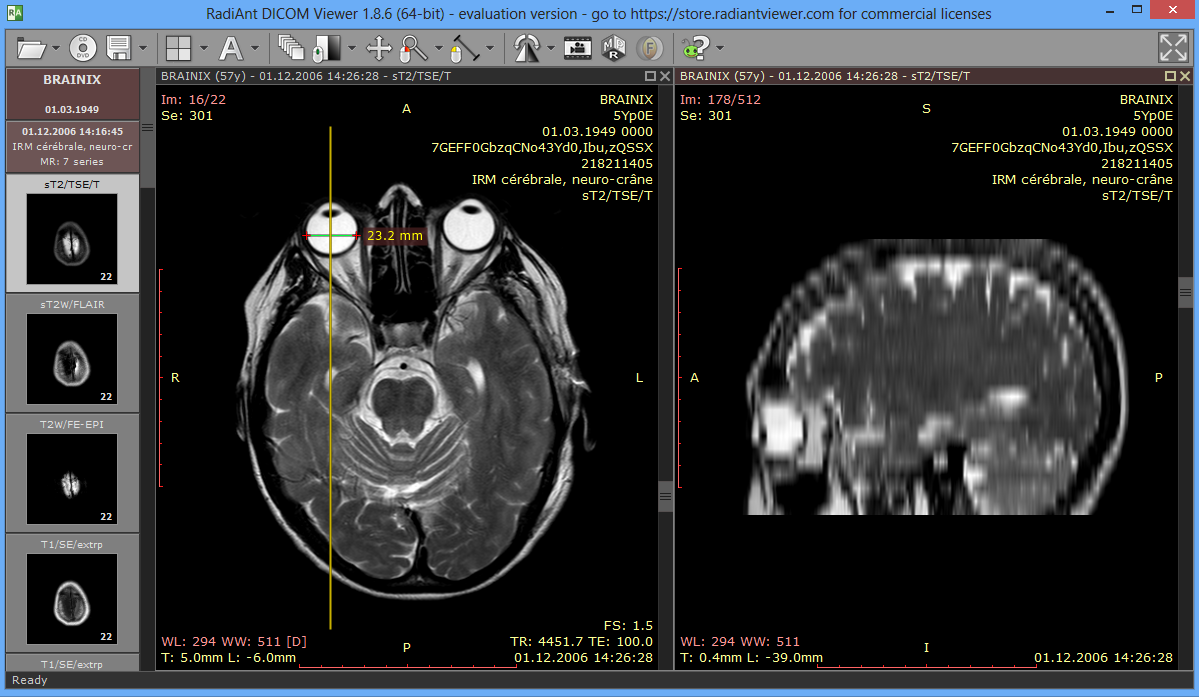
\includegraphics[angle=0,width=9cm]{./img/RadiAnt.png}}
   \caption{RadiAnt - DicomViewer}
  \label{radiant}
  \vspace{0.5cm}
\end{figure}

%\footnotetext{http://www.radiantviewer.com/de/}

% Jetzt eine gleitende Abbildung, die Abbildung wird am oberen 
% Seitenrand positioniert, die Fußnote erhält die Nummer 3
% Der Fußnotenbefehl wird nochmal geschützt

Frei verfügbare Software im medizinischen Bereich beschränkt sich oft in den vom Programm vorgegebenen Funktionen und bietet keine Möglichkeit der Erweiterung. Zusätzlich liegt der Fokus an der Darstellung der Patientenbilder und weniger an den Algorithmen zur Bildverarbeitung. Abbildung \ref{radiant} zeigt den Screenshot des DicomViewers RadiAnt\footnote{http://www.radiantviewer.com/de/}. Die Bilder können einzeln oder wie auf dem Bild zu sehen, im Bezug zueinander betrachtet werden. Die Werkzeugleiste oben ermöglicht die für DICOM-Bilder typischen Operationen.
Zwar gibt es auf dem Markt auch Open-Source Lösungen mit Schwerpunkt auf Bildverarbeitung, jedoch eigenen sich diese nur bedingt für dein Einsatz in der Lehre. Die Programme bieten eine Vielzahl an Funktionen, allerdings benötigt die Entwicklung von Erweiterungen einen erheblichen Zeitaufwand.
 
\begin{figure}[htbp]
  \vspace{0.5cm}
  \centering
  \fbox{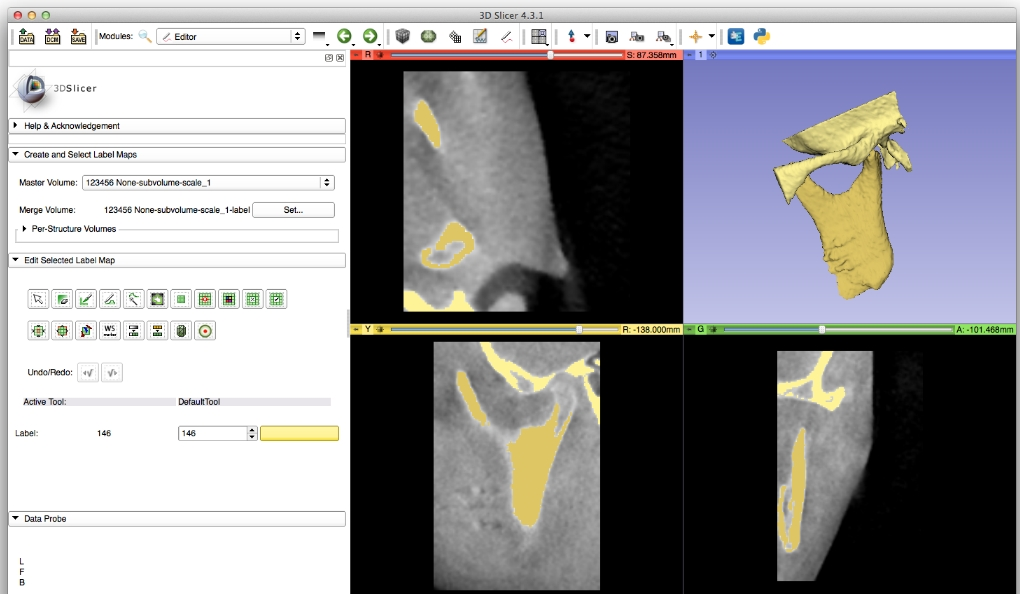
\includegraphics[angle=0,width=9cm]{./img/Screenshot-3DSlicer.png}}
  \floatfoot{Quelle: http://www.linuxlinks.com/portal/content/reviews/Health/Screenshot-3DSlicer.png - abgerufen am 11.01.2014}
  \caption{Screenshot Slicer 3D}
  \label{slicer3d}
  \vspace{0.5cm}
\end{figure}

Slicer 3D\footnote{http://www.slicer.org} (Abbildung \ref{slicer3d}) ist ein umfassendes Werkzeug für die medizinische Bildverarbeitung im zwei- und dreidimensionalen Raum. Die quelloffene Software bietet Möglichkeiten eigene Module zu implementieren. Slicer verwendet als Bibliotheken unter anderem das Insight Toolkit und das Visualization Toolkit\footnote{Insight Toolkit(ITK) und Visualization Toolkit (VTK) sind umfassende Programmbibliotheken zur medizinischen Bildverarbeitung und Visualisierung. Verfasst wurden sie in der Programmiersprache C++}. Das Modul \glqq medizinische Bildverarbeitung\grqq baut auf der Programmiersprache Java auf und ist eine weitere Voraussetzung für einen Einsatz im Lehrgebiet. Module in Slicer werden in Python implementiert. Die Studierenden müssten damit eine zusätzliche Sprache lernen.\\

\begin{figure}[htbp]
  \vspace{0.5cm}
  \centering
  \fbox{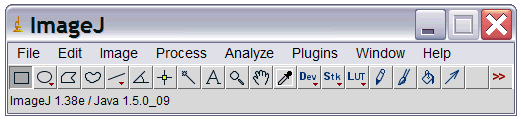
\includegraphics[angle=0,width=9cm]{./img/imagej-window.png}}
  \caption{Die Benutzeroberfläche von ImageJ}
  \floatfoot{ Quelle:  http://rsbweb.nih.gov/ij/features.html - abgerufen am 11.01.2014}
  \label{imagej}
  \vspace{0.5cm}
\end{figure}

\glqq State Of The Art\grqq im Bereich der Bildverarbeitung in Java ist ImageJ\footnote{http://rsbweb.nih.gov/ij/}). Im Grundzustand liefert ImageJ die Standardfunktionen der Bildverarbeitung wie Abbildung \ref{imagej} zeigt. Unter Anderem kann das Bildmaterial analysiert oder mit Filtern bearbeitet werden. ImageJ verarbeitet Grauwertbilder als auch Farbbilder in den gängigen Formaten wie PNG, JPEG und viele andere. Erweiterungen können schnell und zielstrebig entwickelt werden. Im Modul \glqq Bildverarbeitung\grqq der Fakultät Informatik wird ImageJ als Standard zum Bearbeiten der Übungsaufgaben verwendet. Für den Studiengang Biomedizinische Technik fehlt allerdings die grundlegende Unterstützung von medizinischen Bilddaten im DICOM-Format. Die Funktionalität lässt sich über Plug-ins nachträglich hinzufügen, allerdings fehlt eine Bibliothek die bereits implementierte Algorithmen zur Verfügung stellt.

Für eine Software die an der Hochschule Landshut für Lehre sowie Forschung im Bereich der medizinischen Bildverarbeitung eingesetzt werden kann ergeben sich folgende Anforderungen:

\begin{itemize}
\item \textbf{Erweiterbarkeit durch den Anwender} \\
	  Anwender sollen die Möglichkeit haben, das Programm mit selbst programmierten Algorithmen zu erweitern. Die eigene Implementierung von Bildverarbeitungsprozessen ist essentiell im Bereich der Lehre.
\item \textbf{Modularer Aufbau} \\
	  Die Software soll auch in den Grundfunktionen erweiterbar sein, die bei Auslieferung des Programms sofort zur Verfügung stehen (Skalierung, Rotation, etc.). Anders als die von Benutzern erstellten Plug-ins, die abhängig vom Anwender sind muss eine Möglichkeit zur globalen Erweiterung gegeben werden.
\item \textbf{Unterstützung des Dicom-Standards}\\
	  Medizinische Bilddaten besitzen neben den rohen Pixeldaten noch eine Vielzahl zusätzlicher Information wie Patientendaten oder Seriennummern der Aufnahmen und benötigen eine spezielle Verarbeitung. Anders als übliche Grauwertbilder besitzen DICOM-Daten unter Anderem nicht 255 sondern bis zu $2^{16}$ verschiedene Grauwerte.
\item \textbf{Implementierung in der Programmiersprache Java}\\
	  Das Modul zur Bildverarbeitung der Biomedizinischen Technik findet in Java statt. Dadurch wird die Programmiersprache eine Anforderung, da ein Einsatz für die Lehre sonst nur erschwert möglich ist.
\item \textbf{Grundausstattung an medizinischen Bibliotheken}\\
	  Algorithmen in der Bildverarbeitung sind oft komplex und umfangreich. Nicht jeder benötigte Verarbeitungsprozess eignet sich zum selbst implementieren (Sowohl im Lehr- als auch Forschungsbereich). Durch den Einsatz von Bibliotheken wird ein grundlegender Satz an Algorithmen vorgegeben, auf den der Benutzer zurückgreifen und in den Plug-ins verwenden kann.
\end{itemize}

Da in den vorgestellten Anwendungen keine Lösung verfügbar ist die alle Voraussetzungen erfüllt, soll eine Software entwickelt werden, die für das Labor für medizinische Bildverarbeitung, Algorithmen und Krankenhaus IT die benötigten Anforderungen erfüllt.